\documentclass{dcthesis}
\pdfminorversion=7

% Dartmouth thesis template exported from Overleaf and locally adapted only
% for numbered chapter/section headings in dcthesis.cls.

%%%%%%%%%%%%%%%%%%%%%%%%%%%%%%%%%%%%%%%%%%%%%%%%%%
% Defaults
%%%%%%%%%%%%%%%%%%%%%%%%%%%%%%%%%%%%%%%%%%%%%%%%%%
\committee[F. Jon Kull, Ph.D.]{}{}{}{}
\School{Guarini School of Graduate and Advanced Studies}{Dartmouth College}{Hanover, New Hampshire}
\degree{Master of Science}
\field{Computer Science}

%%%%%%%%%%%%%%%%%%%%%%%%%%%%%%%%%%%%%%%%%%%%%%%%%%
% Additional Packages
%%%%%%%%%%%%%%%%%%%%%%%%%%%%%%%%%%%%%%%%%%%%%%%%%%
\usepackage{amsmath,amssymb,amsthm}
\usepackage{array}
\usepackage{graphicx}
\usepackage[colorlinks=true,linkcolor=blue,citecolor=blue,urlcolor=blue]{hyperref}

%%%%%%%%%%%%%%%%%%%%%%%%%%%%%%%%%%%%%%%%%%%%%%%%%%
% Formatting
%%%%%%%%%%%%%%%%%%%%%%%%%%%%%%%%%%%%%%%%%%%%%%%%%%
\renewcommand{\labelenumi}{(\alph{enumi})}
\renewcommand{\labelenumii}{(\roman{enumii})}
\renewcommand{\chaptermark}[1]{\markboth{{\sc #1}}{{\sc #1}}}
\renewcommand{\sectionmark}[1]{\markright{{\sc \thesection\ #1}}}

%%%%%%%%%%%%%%%%%%%%%%%%%%%%%%%%%%%%%%%%%%%%%%%%%%
% Theorem Declarations
%%%%%%%%%%%%%%%%%%%%%%%%%%%%%%%%%%%%%%%%%%%%%%%%%%
\newtheorem{prop}{Proposition}[chapter]
\newtheorem{theorem}[prop]{Theorem}
\newtheorem{lemma}[prop]{Lemma}
\newtheorem{corr}[prop]{Corollary}
\theoremstyle{definition}
\newtheorem{definition}[prop]{Definition}
\theoremstyle{remark}
\newtheorem{remark}[prop]{Remark}
\newtheorem{example}[prop]{Example}
\newtheorem*{claim}{Claim}

%%%%%%%%%%%%%%%%%%%%%%%%%%%%%%%%%%%%%%%%%%%%%%%%%%
% Title Page Information
%%%%%%%%%%%%%%%%%%%%%%%%%%%%%%%%%%%%%%%%%%%%%%%%%%
\title{From Visual Events to Vibrotactile Feedback: A Semantic VAE Pipeline for Temporal Haptic Generation}
\author{Jiayi Liu}
\date{June 2026}
\field{Computer Science}
\degree{Master of Science}
\committee{Nikhil Singh}{Lorie Loeb}{John P. Bell}{}

\begin{document}

%%%%%%%%%%%%%%%%%%%%%%%%%%%%%%%%%%%%%%%%%%%%%%%%%%
% Front Matter
%%%%%%%%%%%%%%%%%%%%%%%%%%%%%%%%%%%%%%%%%%%%%%%%%%
\frontmatter

\newgeometry{left=1.5in,top=1in,bottom=1in,right=1in}
\maketitle
\restoregeometry

\chapter*{Abstract}
\addcontentsline{toc}{section}{Abstract}
[TODO: write the abstract after the main thesis argument and results are finalized.]

\chapter*{Preface}
\addcontentsline{toc}{section}{Preface}
[TODO: write acknowledgments and preface text.]

\tableofcontents

% \listoftables
% \listoffigures

%%%%%%%%%%%%%%%%%%%%%%%%%%%%%%%%%%%%%%%%%%%%%%%%%%
% Main Matter
%%%%%%%%%%%%%%%%%%%%%%%%%%%%%%%%%%%%%%%%%%%%%%%%%%
\mainmatter

\chapter{Introduction}

Vibrotactile feedback can communicate system state, interaction progress, and event salience through short physical sensations. A vibration can confirm success, warn of an error, indicate that a process is ongoing, or draw attention to a notification. Yet designing such feedback remains difficult because haptic meaning depends on temporal structure as much as intensity: onset, duration, rhythm, decay, and repetition all shape how a vibration is perceived.

This challenge is especially clear for temporal visual events. A state transition, loading animation, error cue, or notification arrival is not merely a static visual label; it is an ordered change. A haptic response should therefore fit both the meaning and timing of the event. Recent text-to-vibration systems such as HapticGen show that generative models can support haptic design from natural language prompts~\cite{sung2025hapticgen}. However, prompt-based generation and temporal visual feedback address different needs. A prompt may describe a desired tactile style, but temporal visual events require event-level structure: which moment matters, how the event unfolds, and how tactile feedback should align with that unfolding.

This thesis studies temporal visual haptic generation through UI flows, a common and experimentally controllable class of events in human-computer interaction. The system input is a short sequence of visual states, such as before, during, and after frames for Payment Confirmation, Failed Submission, Notification Received, or Pull to Refresh. These UI flows provide a concrete setting for investigating how visual event meaning can be translated into deployable vibrotactile feedback.

This thesis presents Semantic VAE, a semantic pipeline for generating vibrotactile feedback from temporal visual events. The system first represents a visual transition as one or more semantic haptic events. These event descriptions guide generation through a behavior atlas over the latent space of a convolutional variational autoencoder (VAE). The atlas organizes learned haptic waveforms into interpretable behavior families and supports latent search, while an event timeline mixer composes generated haptic chunks into a coherent two-second response. A shared preprocessing stage then exports the result as an ERM-ready playback sequence.

The central idea is a staged generation pipeline that separates visual-event interpretation, semantic haptic planning, waveform generation, temporal composition, and hardware-oriented export. This structure makes the generation process more stable and inspectable: the system exposes what haptic events were inferred, how they were placed in time, and how they were translated into playable vibration sequences.

I evaluate Semantic VAE in a 27-participant user study using four controlled UI feedback scenarios and five generation strategies: Random Noise, Random-Plan VAE, HapticGen, Direct LLM Pattern, and Semantic VAE. The results show that Semantic VAE provides a stable and competitive generation strategy. It improves perceived meaningfulness over weaker baselines and is selected as the worst stimulus least often, while remaining competitive with stronger generative alternatives. The results also show that visual-event semantics constrain haptic design but do not determine a single preferred vibration pattern: different participants and different visual events favor different balances of salience, rhythm, smoothness, duration, and progress-like feedback.

This thesis makes four contributions:

\begin{enumerate}
    \item A semantic event representation for translating temporal visual events into haptic design decisions.
    \item A behavior-atlas-guided Semantic VAE pipeline for generating haptic feedback through latent search and event timeline composition.
    \item A deployable prototype that converts generated haptic responses into ERM-ready playback sequences for user study evaluation.
    \item Empirical evidence from a 27-participant user study showing that Semantic VAE is stable and competitive while revealing preference-dependent visual-to-haptic mappings.
\end{enumerate}

\chapter{Related Work}

\section{Vibrotactile Feedback and Haptic Meaning}

Vibrotactile feedback is commonly used in interactive systems, but its relevance to this thesis comes from its temporal form. A vibration is not perceived as a static value; it unfolds through onset, duration, rhythm, repetition, and changes in intensity. These temporal properties shape whether a cue feels like confirmation, interruption, progress, or an alert.

Early work on tactons established that brief tactile patterns can serve as structured signals rather than simple on-off alerts. Brewster and Brown define tactons as tactile messages built from parameters such as frequency, amplitude, duration, rhythm, and location~\cite{brewster2004tactons}. For this thesis, the important implication is that haptic meaning depends on organized temporal structure. When the source event is itself temporal, as in a visual state transition, the generated vibration should preserve event-level timing rather than only matching a general tactile style.

\section{Haptic Authoring and Generative Haptics}

Authoring vibrotactile feedback often requires designers to work with temporal patterns, waveform properties, or actuator-level parameters. This can be manageable for a small set of fixed cues, but it becomes difficult to scale when an interface requires many event-specific responses. Temporal visual events add another layer of complexity because the haptic response must reflect not only a general style, but also event meaning, timing, intensity change, and duration.

Recent generative haptic systems aim to reduce this authoring burden. HapticGen generates vibrotactile signals from natural language prompts and frames text as an interface for haptic ideation~\cite{sung2025hapticgen}. ChatHAP extends this direction through a conversational haptic design system that uses a large language model to generate vibrations from signal parameters, navigate libraries, and modify existing vibrations~\cite{lim2025chathap}. Other recent work has explored generative AI for affective vibration, including VAE- and LLM-based models for producing vibrations associated with emotion dimensions such as valence and arousal~\cite{li2025affectivevibration}.

Together, these systems show that generative AI can support vibration authoring, but they also clarify the distinction addressed in this thesis. Existing GenAI haptic systems primarily condition generation on text, conversation, parameters, or affective labels. Temporal visual event feedback requires a representation of event structure before waveform generation: what happened, when it happened, and how tactile feedback should align with the event timeline. Semantic VAE therefore uses a semantic haptic event layer to bridge visual event meaning, haptic generation, and temporal composition.

\section{From Text Prompts to Temporal Visual Events}

Text, conversation, parameters, and affective labels are useful conditioning inputs for haptic generation because they allow users to describe a desired tactile style or communicative intent. However, temporal visual events introduce a different conditioning problem. A visual transition is not only a label such as success, error, or notification; it contains stages, ordering, and moments of emphasis. Compressing such an event into a single prompt risks losing the structure that determines when and how a haptic cue should occur.

Recent work has begun to connect visual or scene context to haptic generation. Scene2Hap uses multimodal large language models to infer object semantics, physical context, material properties, and vibration behavior in VR scenes, then generates scene-wide vibrotactile feedback from those estimates~\cite{jingu2026scene2hap}. This demonstrates the value of visual context for automatic haptic authoring, but it focuses on object-level scene haptics and physical context rather than short temporal visual transitions.

The importance of event structure is also reflected in recent video understanding work. Pang et al. propose a semantic-oriented approach to video temporal localization that represents videos through event and transition structure rather than relying only on boundary timestamps~\cite{pang2026measure}. For this thesis, the relevant implication is that temporal visual inputs often require an intermediate event representation. The problem addressed here is therefore not simply prompt-to-vibration generation, but event-conditioned haptic generation where semantic and temporal structure must be preserved before waveform synthesis.

\section{Semantic Intermediate Representations and Controllable Generation}

Complex generation tasks often benefit from separating high-level semantic decisions from low-level synthesis. Instead of mapping an input description directly to a final artifact, a system can first construct an intermediate representation that captures structure, intent, or constraints. This representation can make generation more inspectable and controllable because users or downstream modules can reason about the intermediate structure before final synthesis.

Text-to-image generation provides a useful analogy. Hong et al. infer a semantic layout from text before synthesizing an image, using the layout as an intermediate representation between language and pixels~\cite{hong2018semanticlayout}. The layout is not the final output, but it exposes spatial and semantic decisions that can guide generation and support user control. The same principle is relevant beyond images: when the target output is a complex signal, an intermediate representation can connect high-level intent to low-level generation.

This thesis applies that idea to vibrotactile feedback for temporal visual events. A direct mapping from a visual prompt to a waveform can hide important decisions about what event occurred, what haptic role it should serve, when the cue should occur, and how it should unfold over time. A semantic haptic event representation makes these decisions explicit before waveform synthesis. It therefore serves as a controllable bridge between visual event semantics and haptic signal generation.

\section{Summary of Gap}

Prior work establishes that vibrotactile meaning depends on temporal structure, that haptic authoring can benefit from generative tools, and that structured intermediate representations can improve controllability in complex generation tasks. Recent systems also show growing interest in connecting language, affective labels, or visual context to haptic output. These directions provide important foundations for this thesis.

However, they do not fully address the problem of generating deployable vibrotactile feedback for short temporal visual events. Existing GenAI haptic systems primarily condition generation on text, conversation, parameters, or affective labels. Visual-to-haptic work has begun to use scene context, but it does not directly address event-level timing in short visual transitions. This thesis therefore focuses on a semantic event representation and generation pipeline that preserve temporal visual structure before waveform synthesis and hardware playback. Chapter 3 describes this Semantic VAE system in detail.

\chapter{System and Methods}

\section{System Overview}

Semantic VAE is a pipeline for generating vibrotactile feedback from temporal visual events. In this thesis, the input events are represented as short UI flows consisting of three visual states: before, during, and after an interaction. These UI flows provide a controlled setting for studying a broader problem: how to translate an ordered visual change into a haptic response that has appropriate meaning, timing, and physical form. The output of the system is a two-second vibrotactile sequence that can be played on an ERM motor through the study prototype.

The system is organized around a semantic intermediate representation rather than a direct mapping from images or prompts to actuator values. Given the three visual states, the system sends the image sequence to an OpenAI 4.1 model with a schema-designed prompt, and the haptic event planner produces an ordered event plan. Each event describes the intended haptic behavior at a higher level, including its behavior class, semantic role, style, strength, timing, and duration. This representation separates the interpretation of the visual event from the synthesis of the final waveform, making it possible to inspect and revise what the system believes the haptic feedback should communicate before generating the low-level signal.

\begin{figure}[t]
\centering
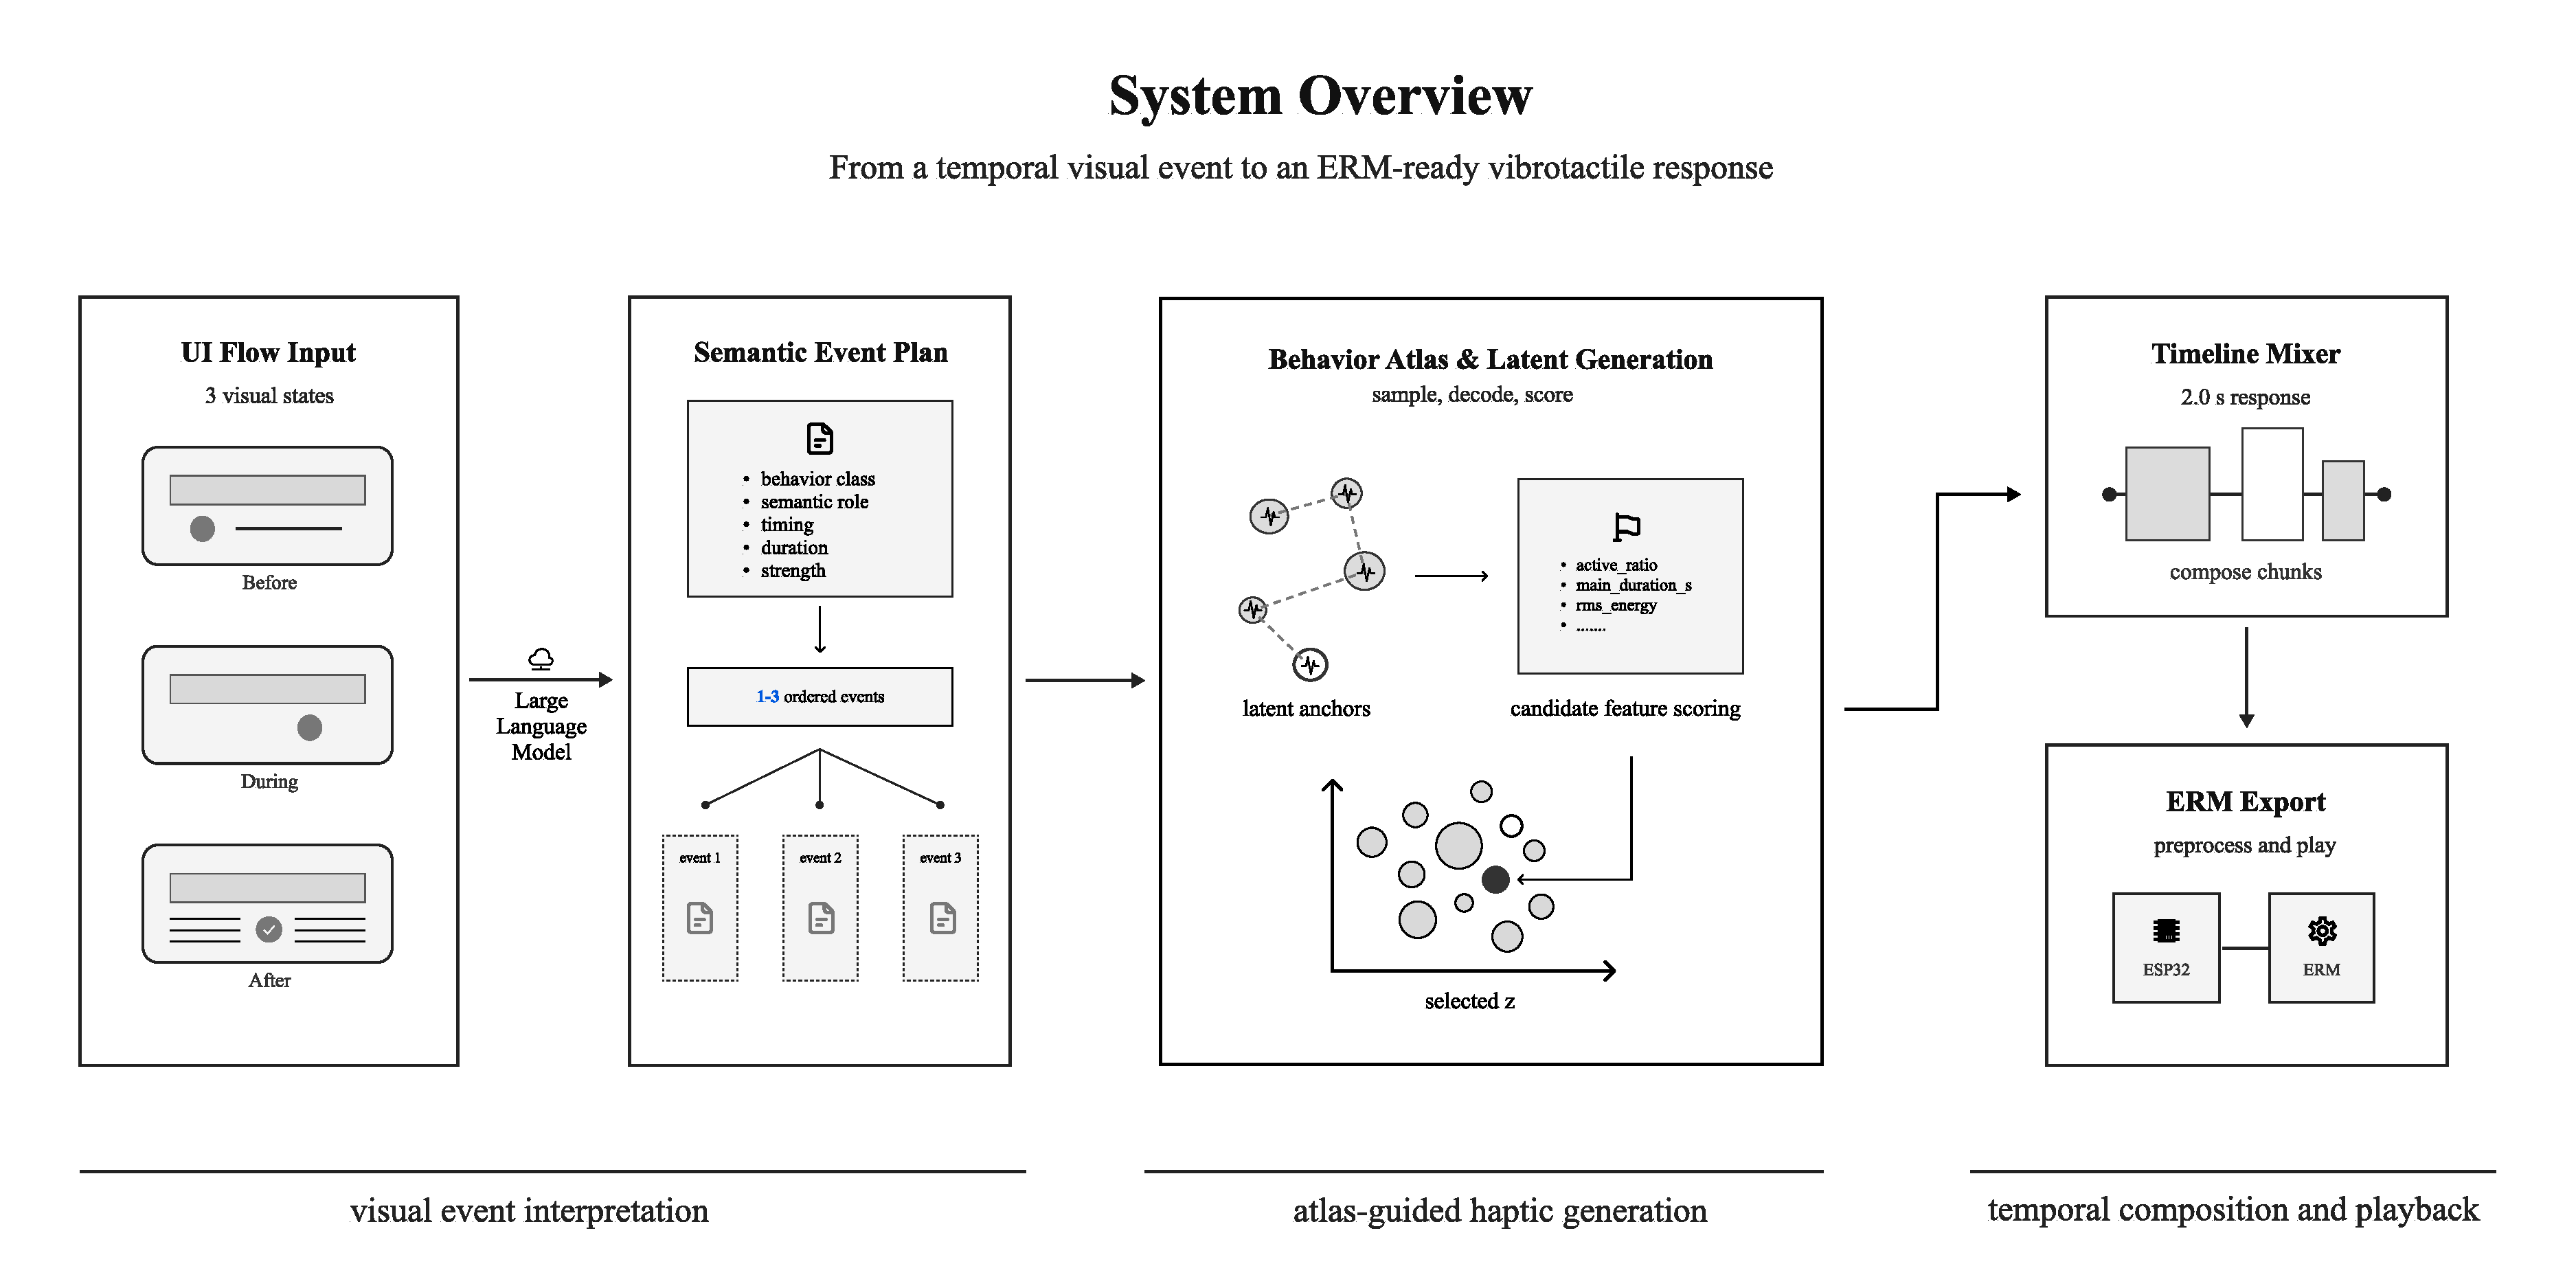
\includegraphics[width=\textwidth]{Figures/system_overview_diagram.pdf}
\caption{Semantic VAE system overview.}
\label{fig:system-overview}
\end{figure}

The event plan then guides waveform generation through a behavior atlas built over a convolutional variational autoencoder (VAE). The atlas groups learned haptic waveforms into interpretable behavior families, such as impacts, ramps, pulses, and other temporal forms. For each planned event, the system converts the semantic description into target waveform features, uses the atlas to identify a plausible region of the VAE latent space, and performs semantic-feature-guided latent search within that region.

Existing waveforms and their latent codes serve as anchors that indicate where similar haptic behaviors are located in the learned space. The system samples candidate latent vectors near those anchors, decodes each candidate with the VAE, measures the resulting waveform features, and selects the generated candidate whose decoded signal best matches the semantic target.

Generated event chunks are passed to an event timeline mixer that composes them into a coherent two-second response. This stage preserves the temporal structure of the visual event by placing each haptic chunk according to the event plan, stretching or shaping chunks as needed, and blending them into a single timeline. Finally, the composed waveform is converted into a hardware-oriented playback sequence using the same ERM preprocessing used for all study stimuli. This final stage accounts for motor constraints and produces a sequence of drive values for playback in the study prototype.

The remainder of this chapter describes each stage of the system in detail: the haptic waveform dataset and VAE model, the behavior atlas, the semantic haptic event representation, latent search, event timeline composition, and ERM export.

\section{Haptic Waveform Dataset and VAE Model}

The VAE provides the generative waveform space used by the rest of the system. It does not interpret the visual input directly. Instead, it learns a latent representation of short vibrotactile waveform chunks, and later stages use semantic planning, atlas structure, and feature-guided latent search to select generated chunks from this learned space. This separation lets the system combine learned haptic signal synthesis with explicit temporal event structure.

The model was trained on 793 WAV files from the HapticGen dataset, split into 634 training files and 159 validation files. Each file was represented during loading by an energy-rich 0.5-second segment sampled at 8 kHz, producing a 4000-sample waveform chunk. The preprocessing pipeline removes the segment mean, normalizes by a global RMS estimate, scales the result by 0.25, and clips values to the range $[-5,5]$. Min--max normalization was disabled. Lightweight augmentation was applied through random gain scaling and small temporal shifts.

\begin{figure}[t]
\centering
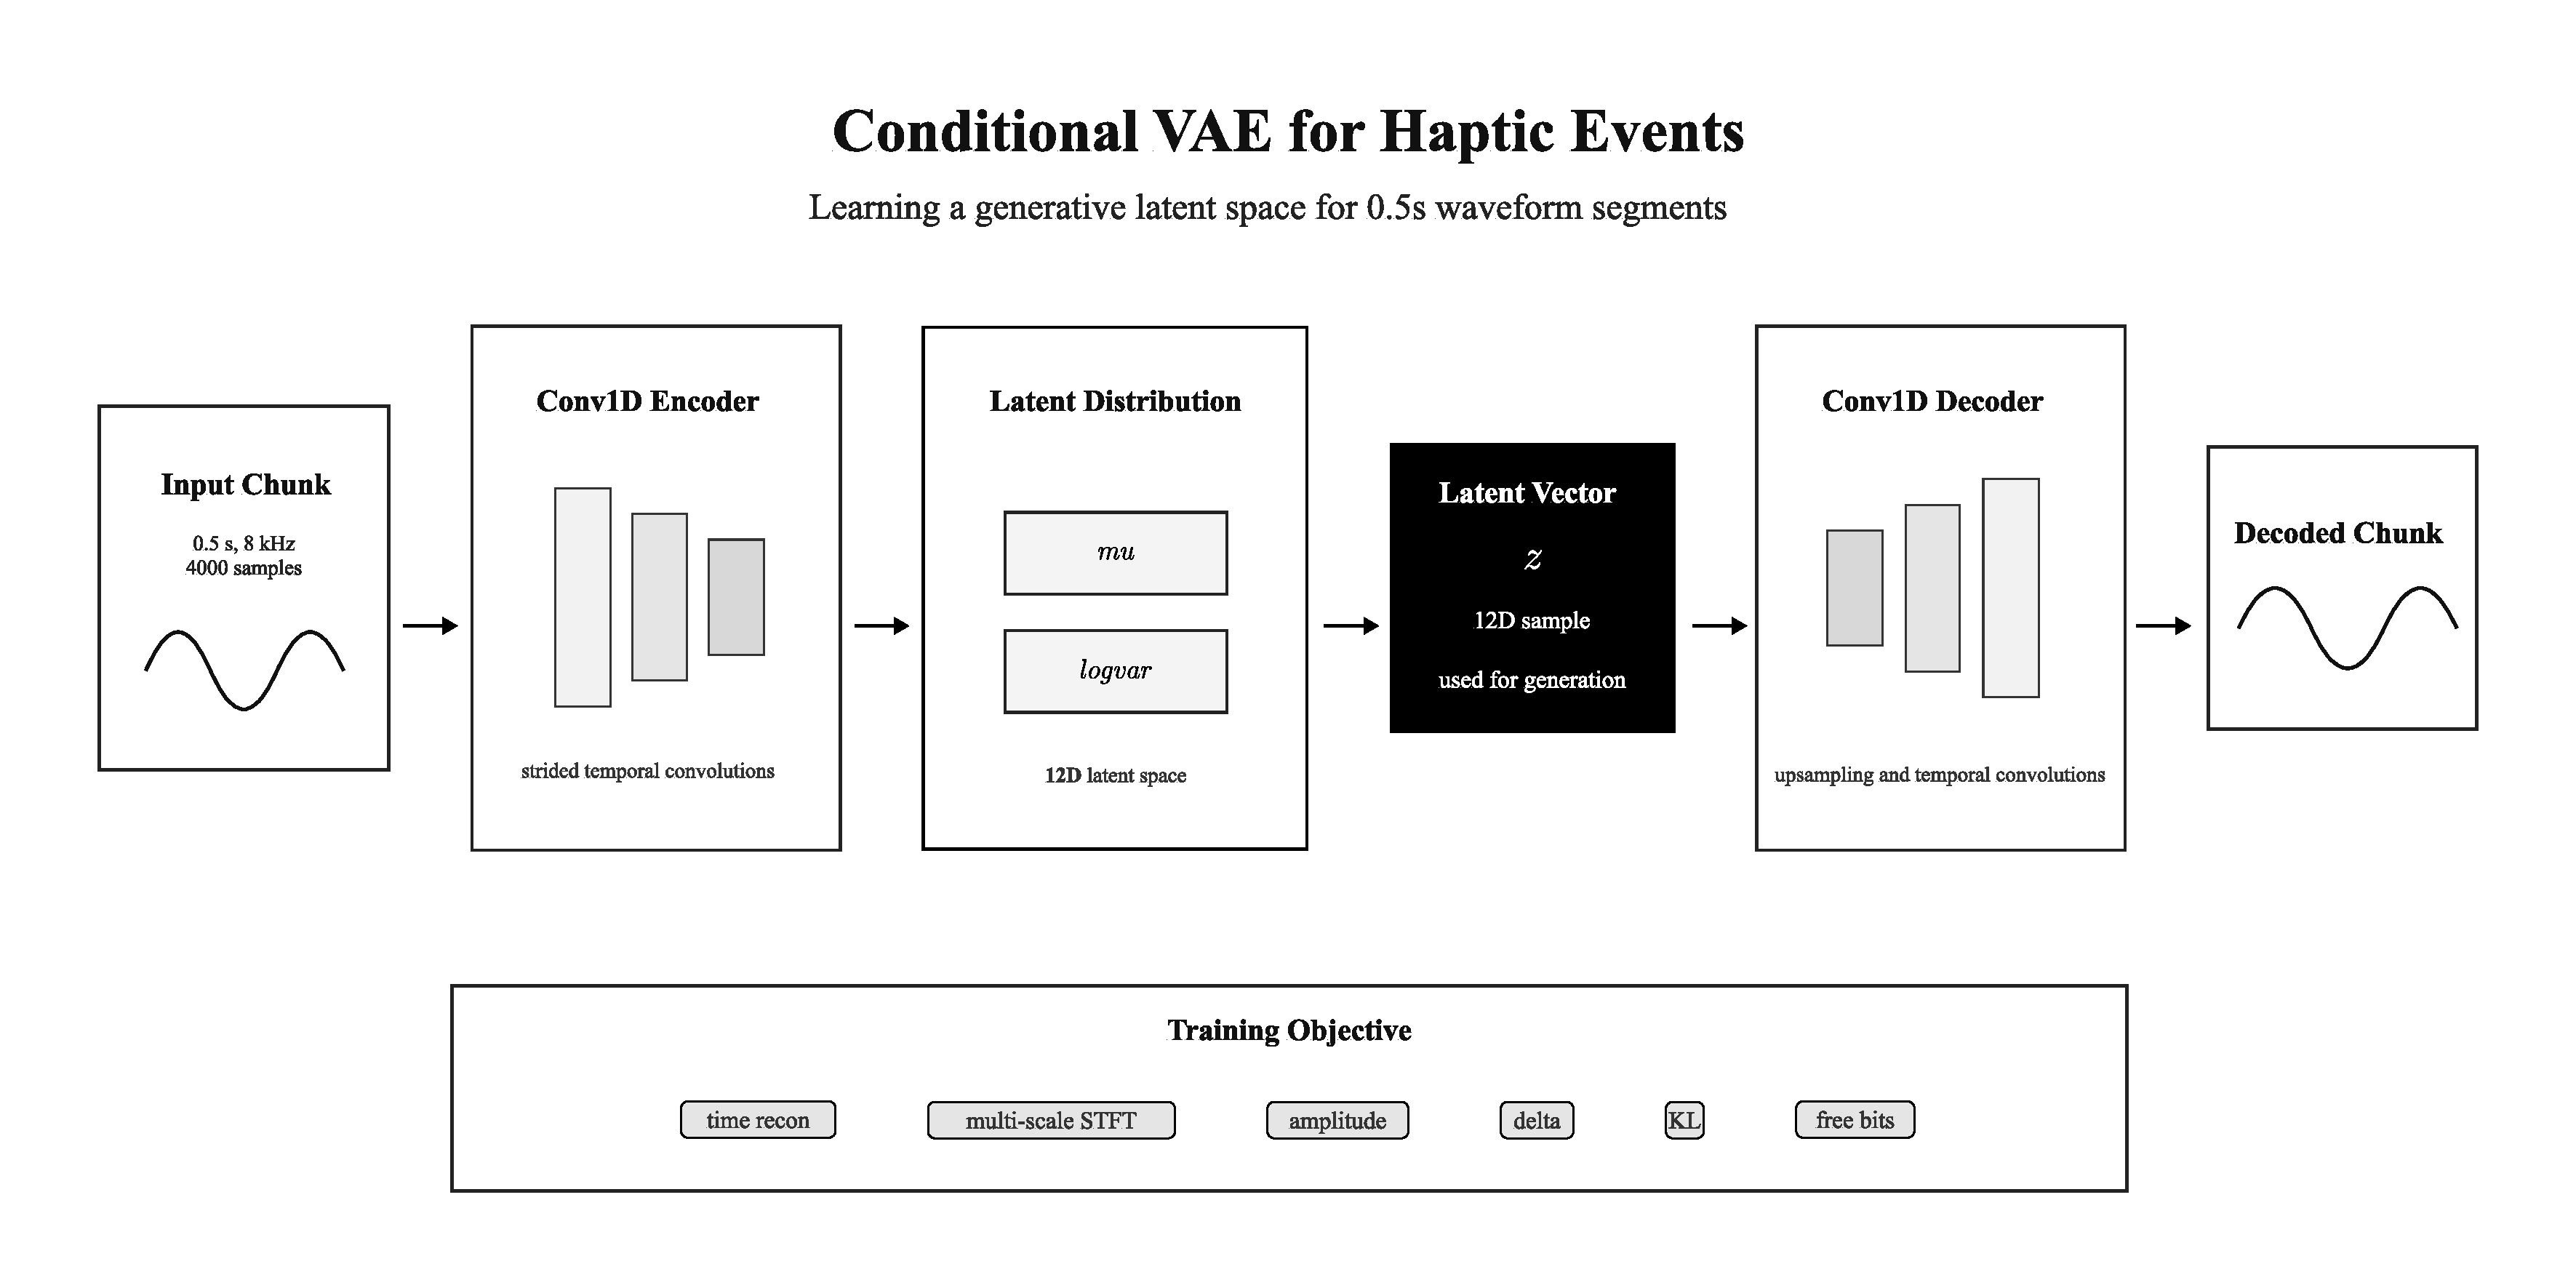
\includegraphics[width=0.95\textwidth]{Figures/conVAE_diagram.pdf}
\caption{Convolutional VAE architecture.}
\label{fig:vae-architecture}
\end{figure}

The model is a one-dimensional convolutional variational autoencoder, shown in Figure~\ref{fig:vae-architecture}. The encoder uses strided temporal convolutions to compress each waveform chunk into a 12-dimensional latent distribution parameterized by $\mu$ and $\log \sigma^2$. Latent vectors sampled from this distribution are passed to a decoder that reconstructs fixed-length waveform chunks using temporal upsampling and convolutional layers. In the generation pipeline, decoded chunks can be produced from candidate latent vectors selected by the atlas-guided search procedure described later in this chapter.

The training objective combines several terms that reflect both signal reconstruction and haptic waveform quality. Time-domain reconstruction encourages sample-level fidelity, while multi-scale STFT terms help preserve spectral structure across short and longer temporal windows. Amplitude, temporal derivative, event-envelope, local-RMS, and onset losses encourage the decoder to preserve properties that are important for vibrotactile perception, such as intensity, transient sharpness, and temporal envelope. KL regularization with free bits maintains a usable latent space for downstream sampling and search. Figure~\ref{fig:vae-training-curve} shows the training curve. Table~\ref{tab:vae-config} summarizes the VAE configuration; the full training configuration is reported in Appendix~\ref{app:system-config}.

\begin{figure}[t]
\centering
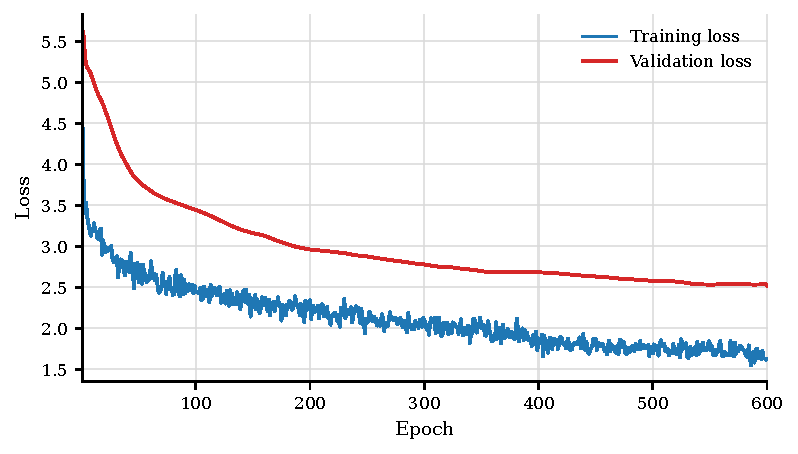
\includegraphics[width=0.78\textwidth]{Figures/vae_training_curve.pdf}
\caption{VAE training curve.}
\label{fig:vae-training-curve}
\end{figure}

\begin{table}[t]
\centering
\caption{Summary of the VAE configuration.}
\label{tab:vae-config}
\renewcommand{\arraystretch}{1.1}
\begin{tabular}{@{}>{\raggedright\arraybackslash}p{1.9in}>{\raggedright\arraybackslash}p{3.9in}@{}}
\hline
\textbf{Item} & \textbf{Configuration} \\
\hline
Dataset & 793 HapticGen WAV files \\
Split & 634 training files and 159 validation files \\
Segment & 0.5 s at 8 kHz; 4000 samples per chunk \\
Preprocessing & Energy-rich segment sampling; global RMS normalization; clipping to $[-5,5]$ \\
Model & One-dimensional convolutional VAE \\
Latent space & 12 dimensions \\
Training & 600 epochs; batch size 16 \\
Loss components & Time-domain reconstruction, multi-scale STFT, amplitude, temporal derivative, event envelope, local RMS, onset, and KL regularization \\
\hline
\end{tabular}
\end{table}


Using 0.5-second chunks rather than full two-second study stimuli is an intentional design choice. Many temporal visual events are composed of local haptic moments: an impact at the moment of confirmation, a short pulse sequence for notification, a rising or falling cue for progress, or a sustained texture for an ongoing state. Short chunks allow the VAE to learn reusable haptic units, while the timeline mixer controls how those units are placed, stretched, and combined into a complete response. The VAE therefore supplies the local generative vocabulary of the system, and later stages impose semantic and temporal structure.

\section{Behavior Atlas}

The behavior atlas organizes the VAE latent space into haptic behavior families that can be used by the semantic generation pipeline. Although the VAE learns a continuous 12-dimensional latent space, the event planner operates in semantic terms such as pulse, ramp, impact, progress, and notification. The atlas provides the bridge between these levels: it groups encoded waveform chunks into interpretable behavior categories, stores class-level latent statistics, and provides curated anchors for later latent search.

The atlas was built from the same 793 HapticGen waveform chunks used to train the VAE. Each chunk was encoded using the deterministic encoder mean $\mu$, producing a 12-dimensional latent vector for every sample. For each waveform, the atlas construction process also computed signal descriptors that capture temporal and spectral behavior, including event count, active duration, RMS energy, peak amplitude, envelope slope, late-to-early energy ratio, amplitude modulation, spectral centroid, onset density, and effective duration. These descriptors support behavior-level organization of the latent space without requiring each latent dimension to have an independent semantic interpretation.

\begin{figure}[t]
\centering
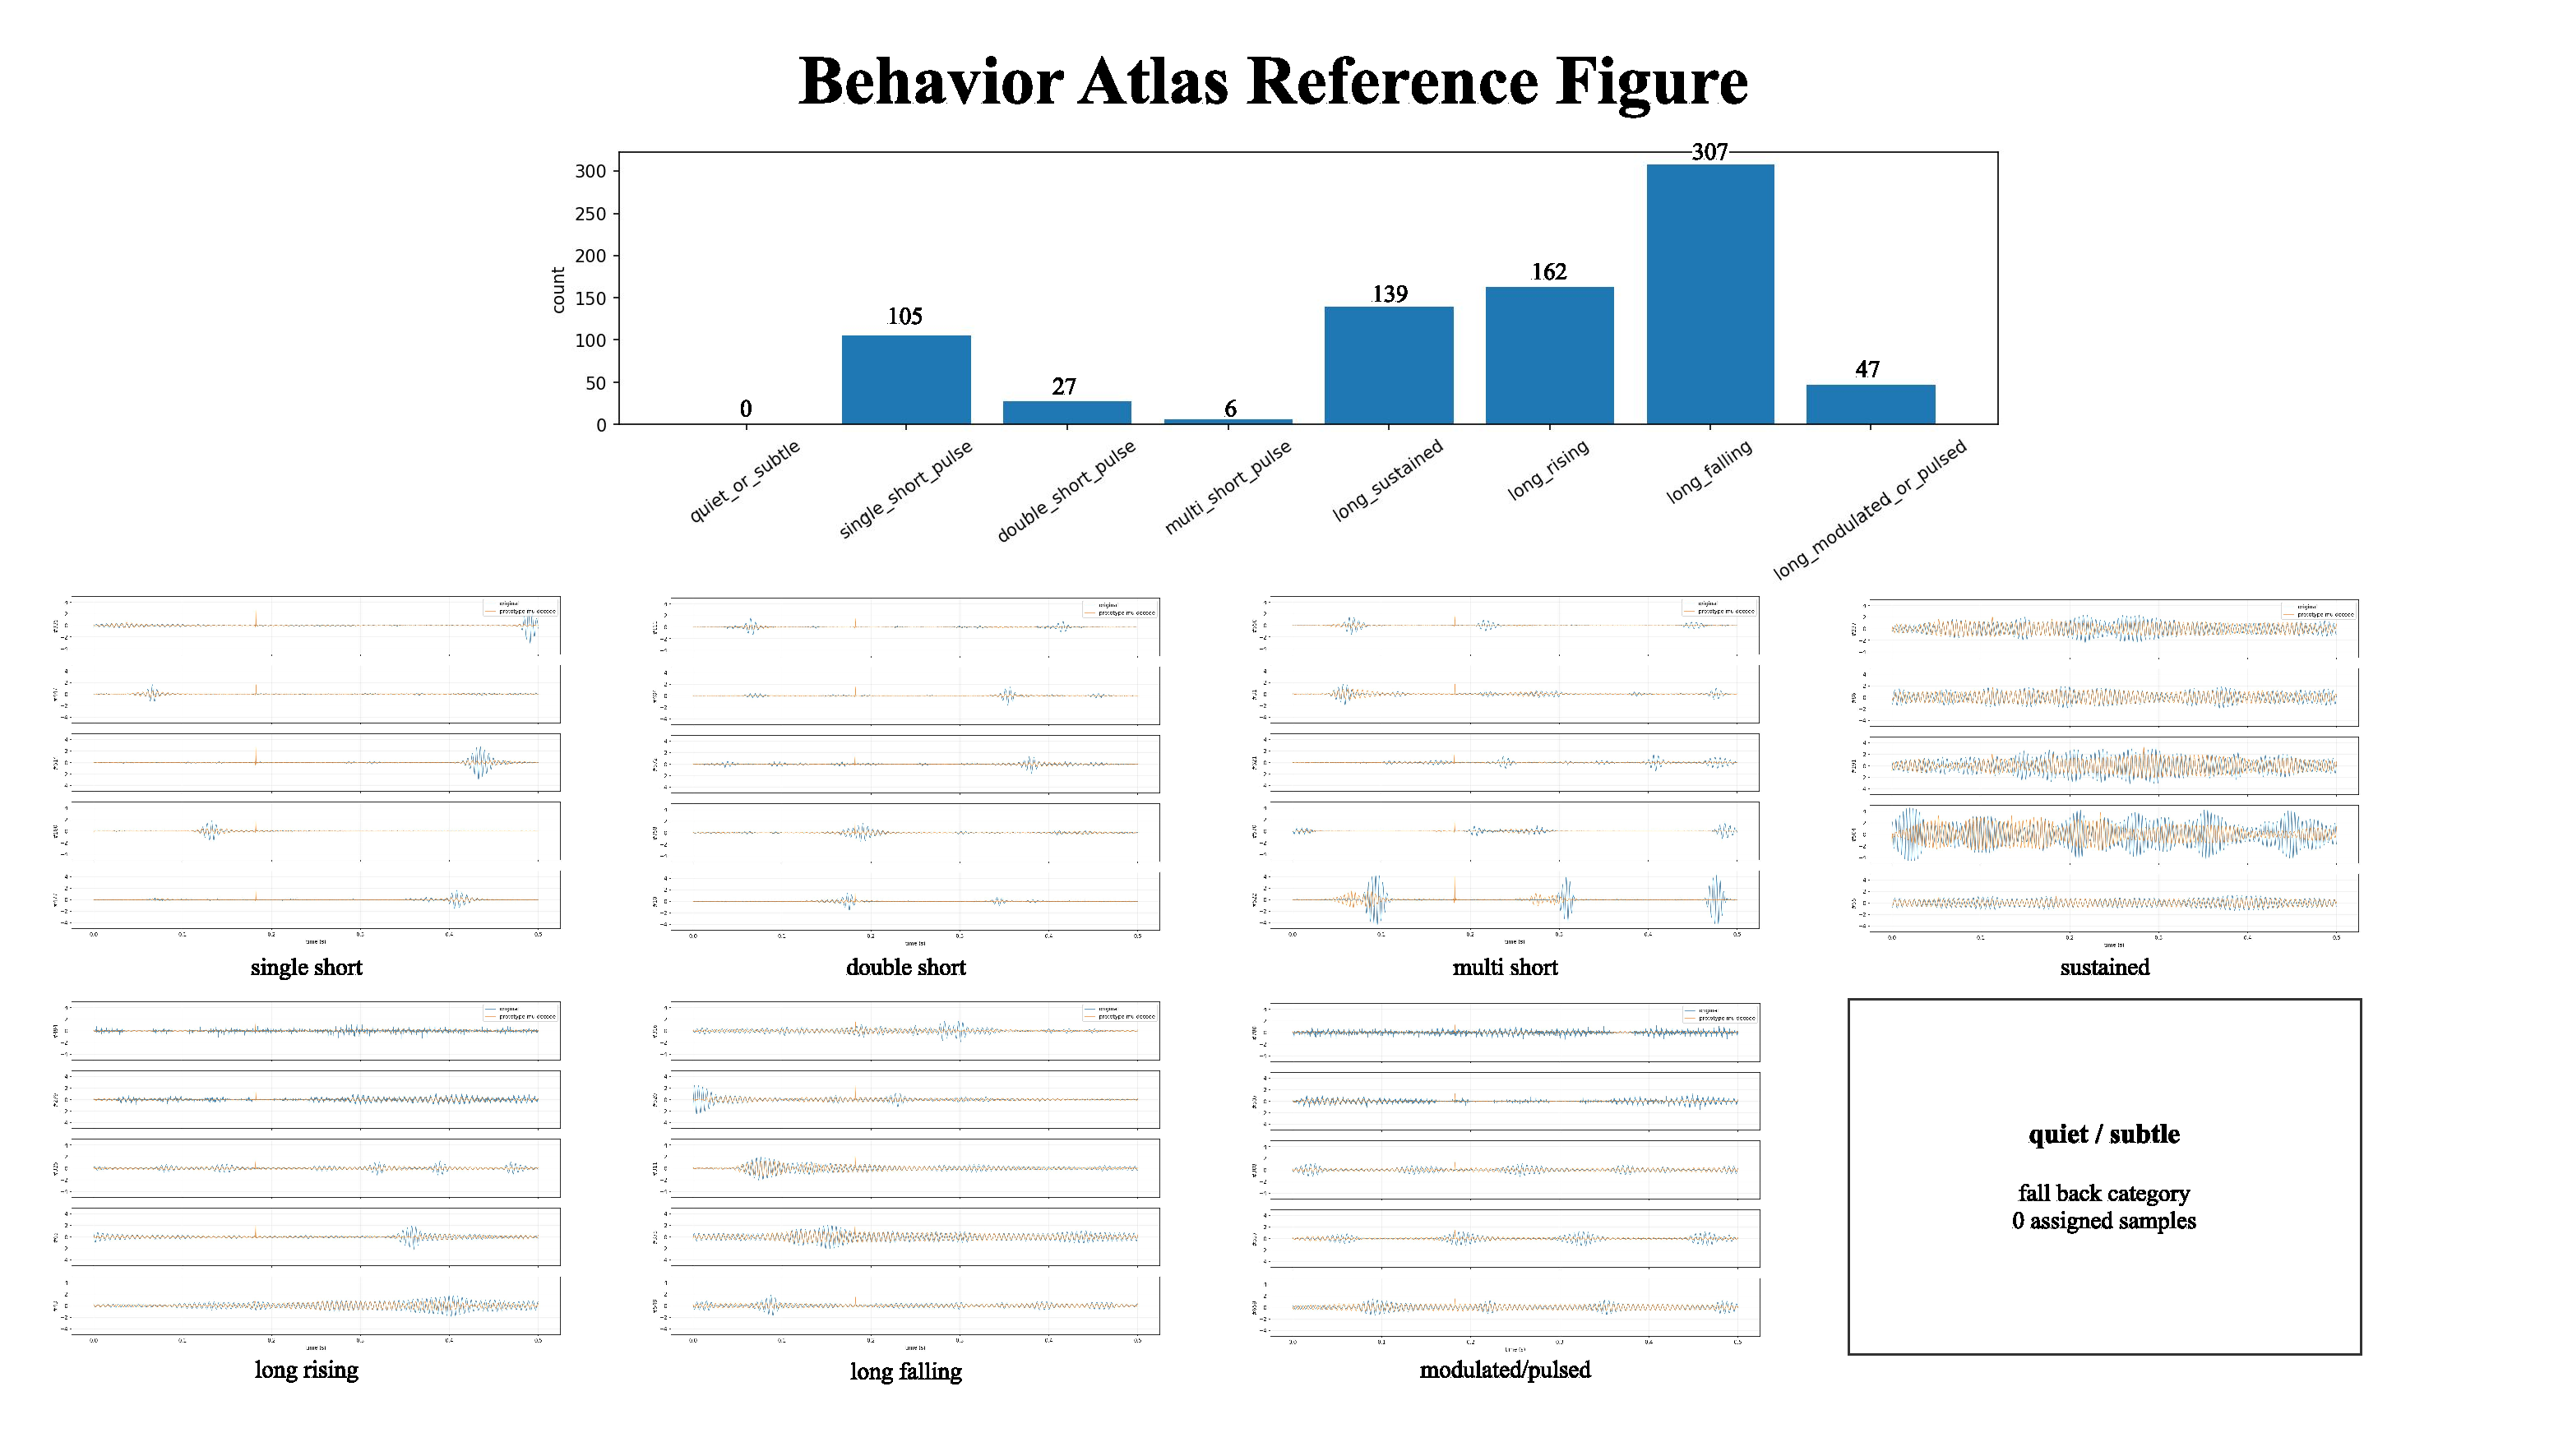
\includegraphics[width=\textwidth]{Figures/atlas_reference.pdf}
\caption{Behavior atlas.}
\label{fig:behavior-atlas}
\end{figure}

The atlas schema contains eight behavior categories: quiet or subtle, single short pulse, double short pulse, multi short pulse, long sustained, long rising, long falling, and long modulated or pulsed. Seven of these categories are represented in the final encoded dataset; quiet or subtle is retained as a fallback category for cases where the planner requests a low-intensity or minimal response. The represented classes are imbalanced, with long falling, long rising, long sustained, and single short pulse forming the largest groups, and multi short pulse appearing least often. Figure~\ref{fig:behavior-atlas} shows the class distribution and representative prototype waveforms.

After automatic feature-based organization, I manually curated the atlas prototypes used by the generation pipeline. For each represented behavior class, I selected a small set of examples that matched the intended temporal behavior. This curation was important because the latent mean of a class does not always decode to a waveform that perceptually belongs to that class. When a candidate near a class center behaved more like another category, I reassigned or excluded it from the curated prototype set. The resulting curated atlas contains two to five approved prototypes for each represented class and serves as a cleaner set of anchors for generation.

In the final system, the atlas is not used as a fixed waveform library. It provides behavior classes, latent regions, prototype anchors, and feature summaries that help the system search within the VAE latent space. When a planned haptic event specifies a behavior class, the atlas identifies a plausible region of the learned haptic manifold and supplies anchors for candidate generation. The next sections describe how the semantic event plan selects these behavior classes and how latent search generates waveform chunks from them.

\section{Semantic Haptic Event Planning}

The semantic haptic event planner converts the three visual states of a UI flow into a structured plan for haptic generation. The input consists of before, during, and after images. These images are sent in order to an OpenAI 4.1 model using a prompt designed around the event schema. The planner uses the images to identify the interaction or state change, summarize the visual transition, and choose one to three ordered haptic events. This stage represents the visual event at the level of haptic intent rather than waveform samples.

In the prototype implementation, the OpenAI 4.1 output is constrained to a fixed JSON schema rather than free-form prose. The schema defines the allowed behavior classes, semantic roles, styles, timing hints, and duration hints used by the rest of the pipeline. The planner returns a JSON object containing an interaction type, a visual change summary, optional composition notes, and an ordered list of haptic events. Each event specifies a communicative role, an atlas behavior class, a qualitative style, an intensity, a coarse timing placement, a coarse duration, and a curated prototype index used as an anchor hint. Table~\ref{tab:semantic-event-schema} summarizes the event fields.

\begin{table}[t]
\centering
\caption{Semantic haptic event schema.}
\label{tab:semantic-event-schema}
\renewcommand{\arraystretch}{1.1}
\begin{tabular}{@{}>{\raggedright\arraybackslash}p{1.45in}>{\raggedright\arraybackslash}p{4.35in}@{}}
\hline
\textbf{Field} & \textbf{Meaning} \\
\hline
\texttt{event\_type} & Visual interaction or state-change type. \\
\texttt{semantic\_role} & Communicative haptic role, such as press, drag, release, confirmation, notification, warning, state change, or subtle context. \\
\texttt{behavior\_class} & Behavior atlas category used to route the event to a latent search region. \\
\texttt{style} & Qualitative haptic style, such as soft, sharp, strong, smooth, ticked, bumpy, rising, falling, sustained, or subtle. \\
\texttt{strength} & Intended intensity on a continuous scale from 0.0 to 1.0. \\
\texttt{timing\_hint} & Coarse temporal placement: beginning, middle, or end. \\
\texttt{duration\_hint} & Coarse duration: short, medium, long, or full. \\
\texttt{prototype\_index} & Curated atlas anchor hint used by latent search. \\
\texttt{reason} & Short planner rationale for the event. \\
\hline
\end{tabular}
\end{table}


The schema uses closed option sets for the main semantic fields. Semantic roles include press-down, drag, pull, scroll, release, confirmation, notification, warning, state change, and subtle context. Style options include soft, sharp, strong, smooth, ticked, bumpy, rising, falling, sustained, and subtle. Timing hints are limited to beginning, middle, and end. Duration hints are mapped to approximate durations: short to 0.5 seconds, medium to 0.8 seconds, long to 1.2 seconds, and full to 2.0 seconds. Strength is represented as a numeric value between 0.0 and 1.0.

The planner output is intentionally higher-level than the waveform generator. It does not assign exact latent vectors or final waveform samples. Instead, it expresses what haptic behavior should occur, why it should occur, and where it should be placed within the event sequence. The prototype index is interpreted as a curated atlas anchor hint for downstream search, while the final latent vector is selected by the semantic-feature-guided search procedure described in the next section.

For example, in an error-flow stimulus where the user checks a ``Delete My Account'' option and an error modal appears, the planner produced two haptic events. The first event represented the initial press-down interaction as a sharp single short pulse at the beginning of the timeline. The second represented the later error state change as a stronger double short pulse near the end. This plan preserves the temporal structure of the visual event before waveform generation: an initial input action followed by a later system response.

Although this thesis uses UI flows as the controlled input domain, the planner is the main domain-specific component of the pipeline. Other temporal visual event domains could use the same downstream VAE, atlas, latent search, and timeline mixer if their visual events are mapped into the same semantic haptic event representation or an adapted schema.

\section{Semantic-Feature-Guided Latent Search}

Each semantic haptic event is converted into a generated latent vector through a feature-based search. The event plan defines the intended haptic behavior, the atlas locates relevant regions of the VAE latent space, and decoded waveform features determine the final candidate. Implementation parameters for this stage are reported in Appendix~\ref{app:system-config}.

The search begins by converting the event fields into target waveform features. Given a semantic haptic event $e$, the system constructs an event-derived target vector

\begin{equation}
\mathbf{t} = g(e).
\end{equation}

This target vector is initialized from the feature statistics of the requested behavior class and then adjusted according to the semantic role, style, strength, and duration hint. The target features include event count, active ratio, main event duration, RMS energy, crest factor, amplitude modulation, envelope slope, envelope decay, and spectral centroid. For example, a double short pulse event encourages two active events, while a strong or sharp style increases target energy, crest factor, and spectral centroid.

\begin{figure}[t]
\centering
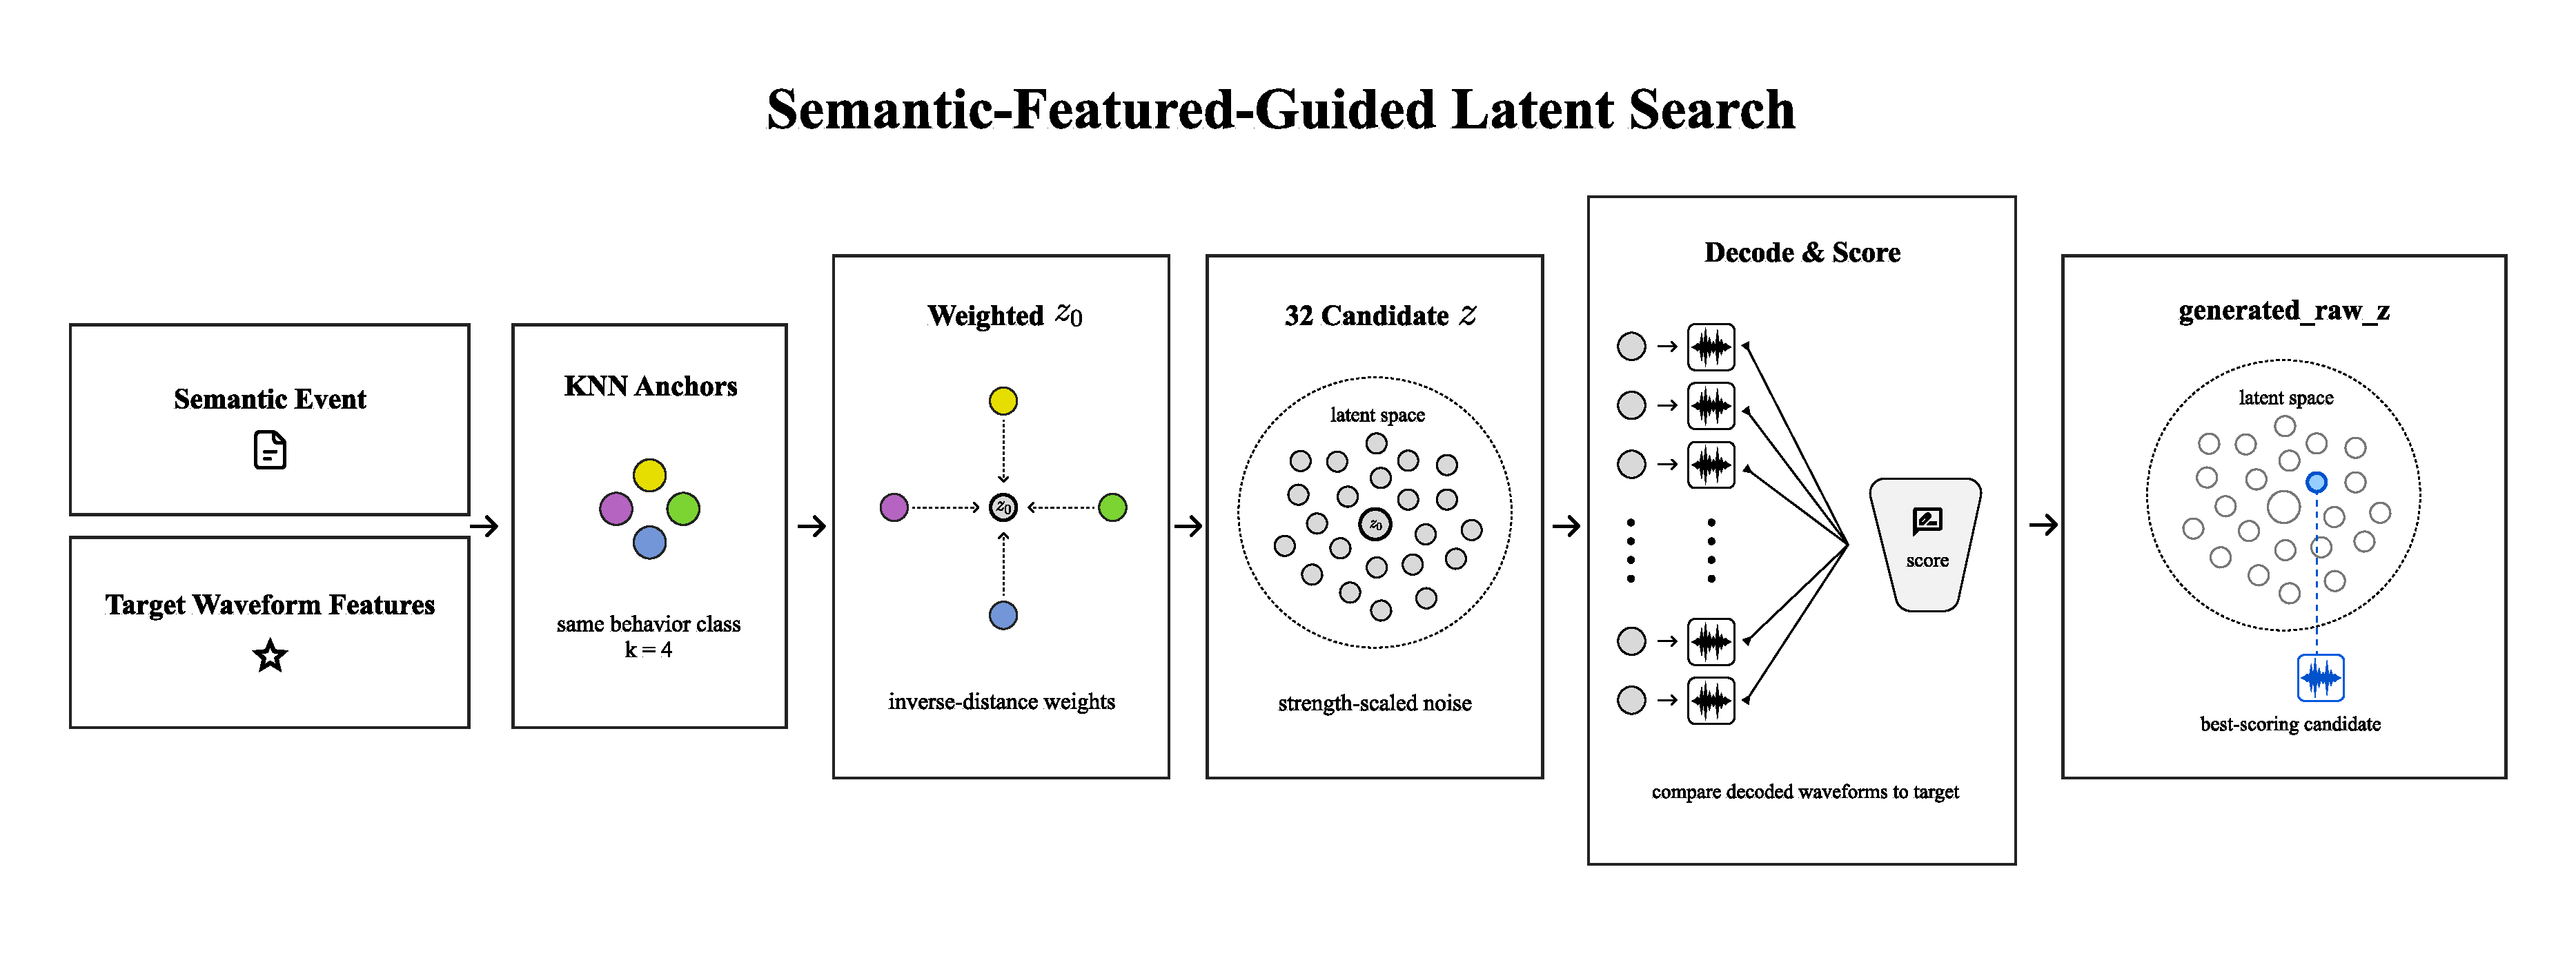
\includegraphics[width=\textwidth]{Figures/latent_search.pdf}
\caption{Semantic-feature-guided latent search.}
\label{fig:latent-search}
\end{figure}

Within the requested behavior class, the system compares the target feature vector against the curated atlas prototypes for that class. The four nearest prototypes are selected as anchors. The user-facing \texttt{prototype\_index} from the event plan biases this anchor selection toward the requested curated example, but the anchors define the local search region rather than the final objective. The objective is the event-derived target vector $\mathbf{t}$. Distances are computed over standardized waveform features with feature-specific weights:

\begin{equation}
D(\mathbf{x}, \mathbf{t}) =
\sqrt{
\sum_m \alpha_m
\left(
\frac{f_m(\mathbf{x}) - t_m}{\sigma_m}
\right)^2
},
\end{equation}

where $f_m(\mathbf{x})$ is feature $m$ of waveform or prototype $\mathbf{x}$, $t_m$ is the semantic target value, $\sigma_m$ is the class-specific feature scale, and $\alpha_m$ is the feature weight.

The selected anchors are weighted by inverse distance. Given anchor latents $\mathbf{z}_i$ and distances $d_i$, the anchor weights and initial latent estimate are

\begin{equation}
w_i =
\frac{1/(d_i+\epsilon)}
{\sum_j 1/(d_j+\epsilon)},
\qquad
\mathbf{z}_0 = \sum_{i=1}^{k} w_i \mathbf{z}_i ,
\end{equation}

with $k=4$. The system then samples 32 candidate latent vectors around $\mathbf{z}_0$. The sampling noise is scaled by the local latent variation of the selected anchors and by the requested event strength:

\begin{equation}
\mathbf{z}_c =
\mathbf{z}_0 +
\boldsymbol{\eta}_c \odot \boldsymbol{\sigma}_{\mathrm{local}}
\sigma_{\mathrm{cand}},
\qquad
\sigma_{\mathrm{cand}} = \lambda(0.45 + 0.75s),
\end{equation}

where $\boldsymbol{\eta}_c$ is standard normal noise, $\boldsymbol{\sigma}_{\mathrm{local}}$ is the local latent standard deviation, $s$ is the event strength, and $\lambda$ is the base candidate noise scale. In this implementation, $\lambda=0.20$, so stronger events search a wider local region around the anchor estimate. Candidate latents are clipped to the class-specific latent range when quantile clipping is enabled.

Each candidate latent vector is decoded by the VAE into a waveform chunk. The scoring step is performed after decoding, so the selection criterion is based on the waveform that the candidate actually generates. For each decoded candidate, the system recomputes the same feature set used in the target representation and compares those features against $\mathbf{t}$. The selected event latent is therefore

\begin{equation}
\mathbf{z}^{*}
=
\arg\min_{\mathbf{z}_c \in \mathcal{Z}_{\mathrm{cand}}}
D\left(F\left(\mathrm{Dec}(\mathbf{z}_c)\right), \mathbf{t}\right),
\end{equation}

where $F$ extracts waveform features and $\mathrm{Dec}$ is the VAE decoder. The best candidate $\mathbf{z}^{*}$ is stored as \texttt{generated\_raw\_z} and decoded into the haptic chunk passed to the timeline mixer.

\section{Event Timeline Mixer}

The event timeline mixer converts the generated event chunks into a fixed two-second haptic response. Each event chunk is produced independently by the VAE decoder, but temporal visual events often contain multiple moments, such as an input action followed by a system response. The mixer preserves this event structure by assigning each generated chunk a duration and position within a shared timeline before producing the final waveform.

The mixer operates at the same sample rate as the VAE, 8 kHz, and produces a final waveform of 16000 samples. Each planned event enters the mixer with a duration hint that has already been mapped to seconds: short, medium, long, or full. If the planned events and gaps fit within the two-second window, those preferred durations are used directly. If they exceed the available time, the mixer first compresses longer events while respecting a minimum event duration, then reduces the inter-event gap if needed, and finally scales all event durations as a fallback.

Each decoded chunk is shaped before placement. The waveform is stretched or held to match the assigned duration using the hold-stretch duration mode. The event strength $s$ is converted to an amplitude gain,

\begin{equation}
g = 0.5 + 0.8s,
\end{equation}

so stronger planned events produce larger waveform amplitudes before clipping. A 10 ms fade is applied at event boundaries to reduce abrupt transitions between silence and vibration.

Timeline placement is determined by event order, timing hints, and alignment rules. Events are separated by a default 0.08-second gap. If the first event is marked as beginning, the sequence starts at the beginning of the two-second response. If the final event is marked as end, or if its role is confirmation, release, notification, or warning, the sequence is aligned so that the event sequence ends near 1.9 seconds. Otherwise, the event sequence is centered in the two-second window. These rules provide deterministic placement while preserving the coarse timing decisions made by the planner.

The mixer combines scheduled chunks additively into the final waveform and clips the result to the configured amplitude range. In the final stimulus generation run, the mixed waveform was clipped to $\pm 3.0$. The output of this stage is still an 8 kHz waveform; the next export stage converts it into a 10 ms interval sequence for ERM playback.

\section{ERM Preprocessing and Export}

The timeline mixer outputs a two-second waveform at 8 kHz, but the study prototype plays discrete motor drive values rather than audio-rate waveform samples. The export stage therefore converts the mixed waveform into a 10 ms interval sequence with 200 values over the same two-second duration. This sequence represents the intended drive envelope for the actuator, not an audio signal.

The ERM preprocessing stage then converts the 10 ms sequence into a hardware-ready 20 ms interval sequence with 100 values. The conversion uses peak-hold resampling from 10 ms to 20 ms so that short peaks are preserved when the sequence is downsampled. Low values below the motor threshold are removed, and the remaining values are remapped with a gamma curve into a bounded drive range. The preprocessing also extends very short nonzero pulses and applies short attack and release smoothing so that events remain perceivable on an ERM motor.

This preprocessing is important because ERM motors have physical inertia and a practical activation threshold. Very brief or low-amplitude changes in a raw sequence may not produce reliable tactile sensations, while abrupt changes can feel inconsistent across stimuli. The preprocessing stage makes the generated sequence more compatible with the actuator while preserving the event timing produced by the earlier pipeline stages.

All five methods compared in the user study use this same export and ERM preprocessing pipeline. Random Noise, Random VAE, HapticGen, Direct LLM Pattern, and Semantic VAE each produce a two-second, 10 ms interval sequence before preprocessing, and each is converted into the same 20 ms interval ERM-ready format. The user study therefore compares the haptic generation methods under a shared playback representation rather than under method-specific actuator processing.

Together, these stages define the final generation method evaluated in this thesis. The system represents visual transitions as semantic haptic events, uses the behavior atlas to guide generation in the VAE latent space, composes generated chunks into a fixed temporal response, and exports that response through a shared ERM playback format. The next chapter describes how this method was evaluated against alternative generation baselines in a controlled user study.

\chapter{Prototype and User Study}

\section{Prototype Interface and Playback Setup}

To evaluate the generated haptic stimuli, I built a browser-based panel of stimuli that presented each visual event together with a set of anonymous vibration options. The prototype was designed as an evaluation interface rather than a real-time generation interface: all haptic stimuli were generated before the study, converted into ERM-ready playback sequences, and loaded onto the study hardware. During the study, the prototype provided a controlled way for participants to experience, replay, rate, and compare those stimuli.

\begin{figure}[!htbp]
\centering
\fbox{\parbox[c][2.2in][c]{0.88\textwidth}{\centering [TODO: insert prototype interface screenshot]}}
\caption{Prototype interface.}
\label{fig:study-prototype}
\end{figure}

For each study block, the browser displayed one fixed UI flow and a panel of anonymous haptic cards, as shown in Figure~\ref{fig:study-prototype}. Participants clicked the cards themselves to trigger individual stimuli. Selecting a card replayed the same visual flow while sending the anonymous stimulus ID to the haptic device through the Web Serial API. This design kept the visual event constant within a block, so differences in participant ratings were attributable to the haptic stimulus rather than changes in the visual presentation.

\begin{figure}[!htbp]
\centering
\fbox{\parbox[c][2.2in][c]{0.88\textwidth}{\centering [TODO: insert hardware playback diagram]}}
\caption{Hardware playback setup.}
\label{fig:hardware-playback}
\end{figure}

The hardware path was the same for every stimulus, as summarized in Figure~\ref{fig:hardware-playback}. A browser event sent the selected anonymous ID over serial to an ESP32, which selected the corresponding stored sequence and streamed it to a DRV2605L haptic driver in real-time playback mode. The driver controlled an ERM motor using the 20 ms interval drive values described in Chapter 3. Participants held the ERM motor directly between their fingers while viewing the prototype, allowing them to feel each vibration as the visual flow played.

The interface allowed flexible exploration within each flow block. Participants could experience the anonymous haptic cards in any order, replay a stimulus as many times as they wanted, and revise their ratings before moving to the next flow. After rating the individual stimuli, participants completed a block-level comparison on the same page, selecting one to three best-matching haptics and one to three worst-matching haptics and optionally explaining their choices in text. Method labels were hidden throughout the study, so participants only saw anonymous stimulus IDs rather than the generation method that produced each vibration.

\section{Study Stimuli}

The study used four controlled UI flows as representative temporal visual events: Payment Confirmation, Failed Submission, Notification Received, and Pull to Refresh. Each flow was designed as a controlled Figma prototype and then implemented in the browser panel with fixed timing, as shown in Figure~\ref{fig:study-ui-flows}. These flows were selected to cover common interaction feedback cases while placing different demands on the haptic response: success confirmation, error salience, notification arrival, and loading or progress feedback.

\begin{figure}[!htbp]
\centering
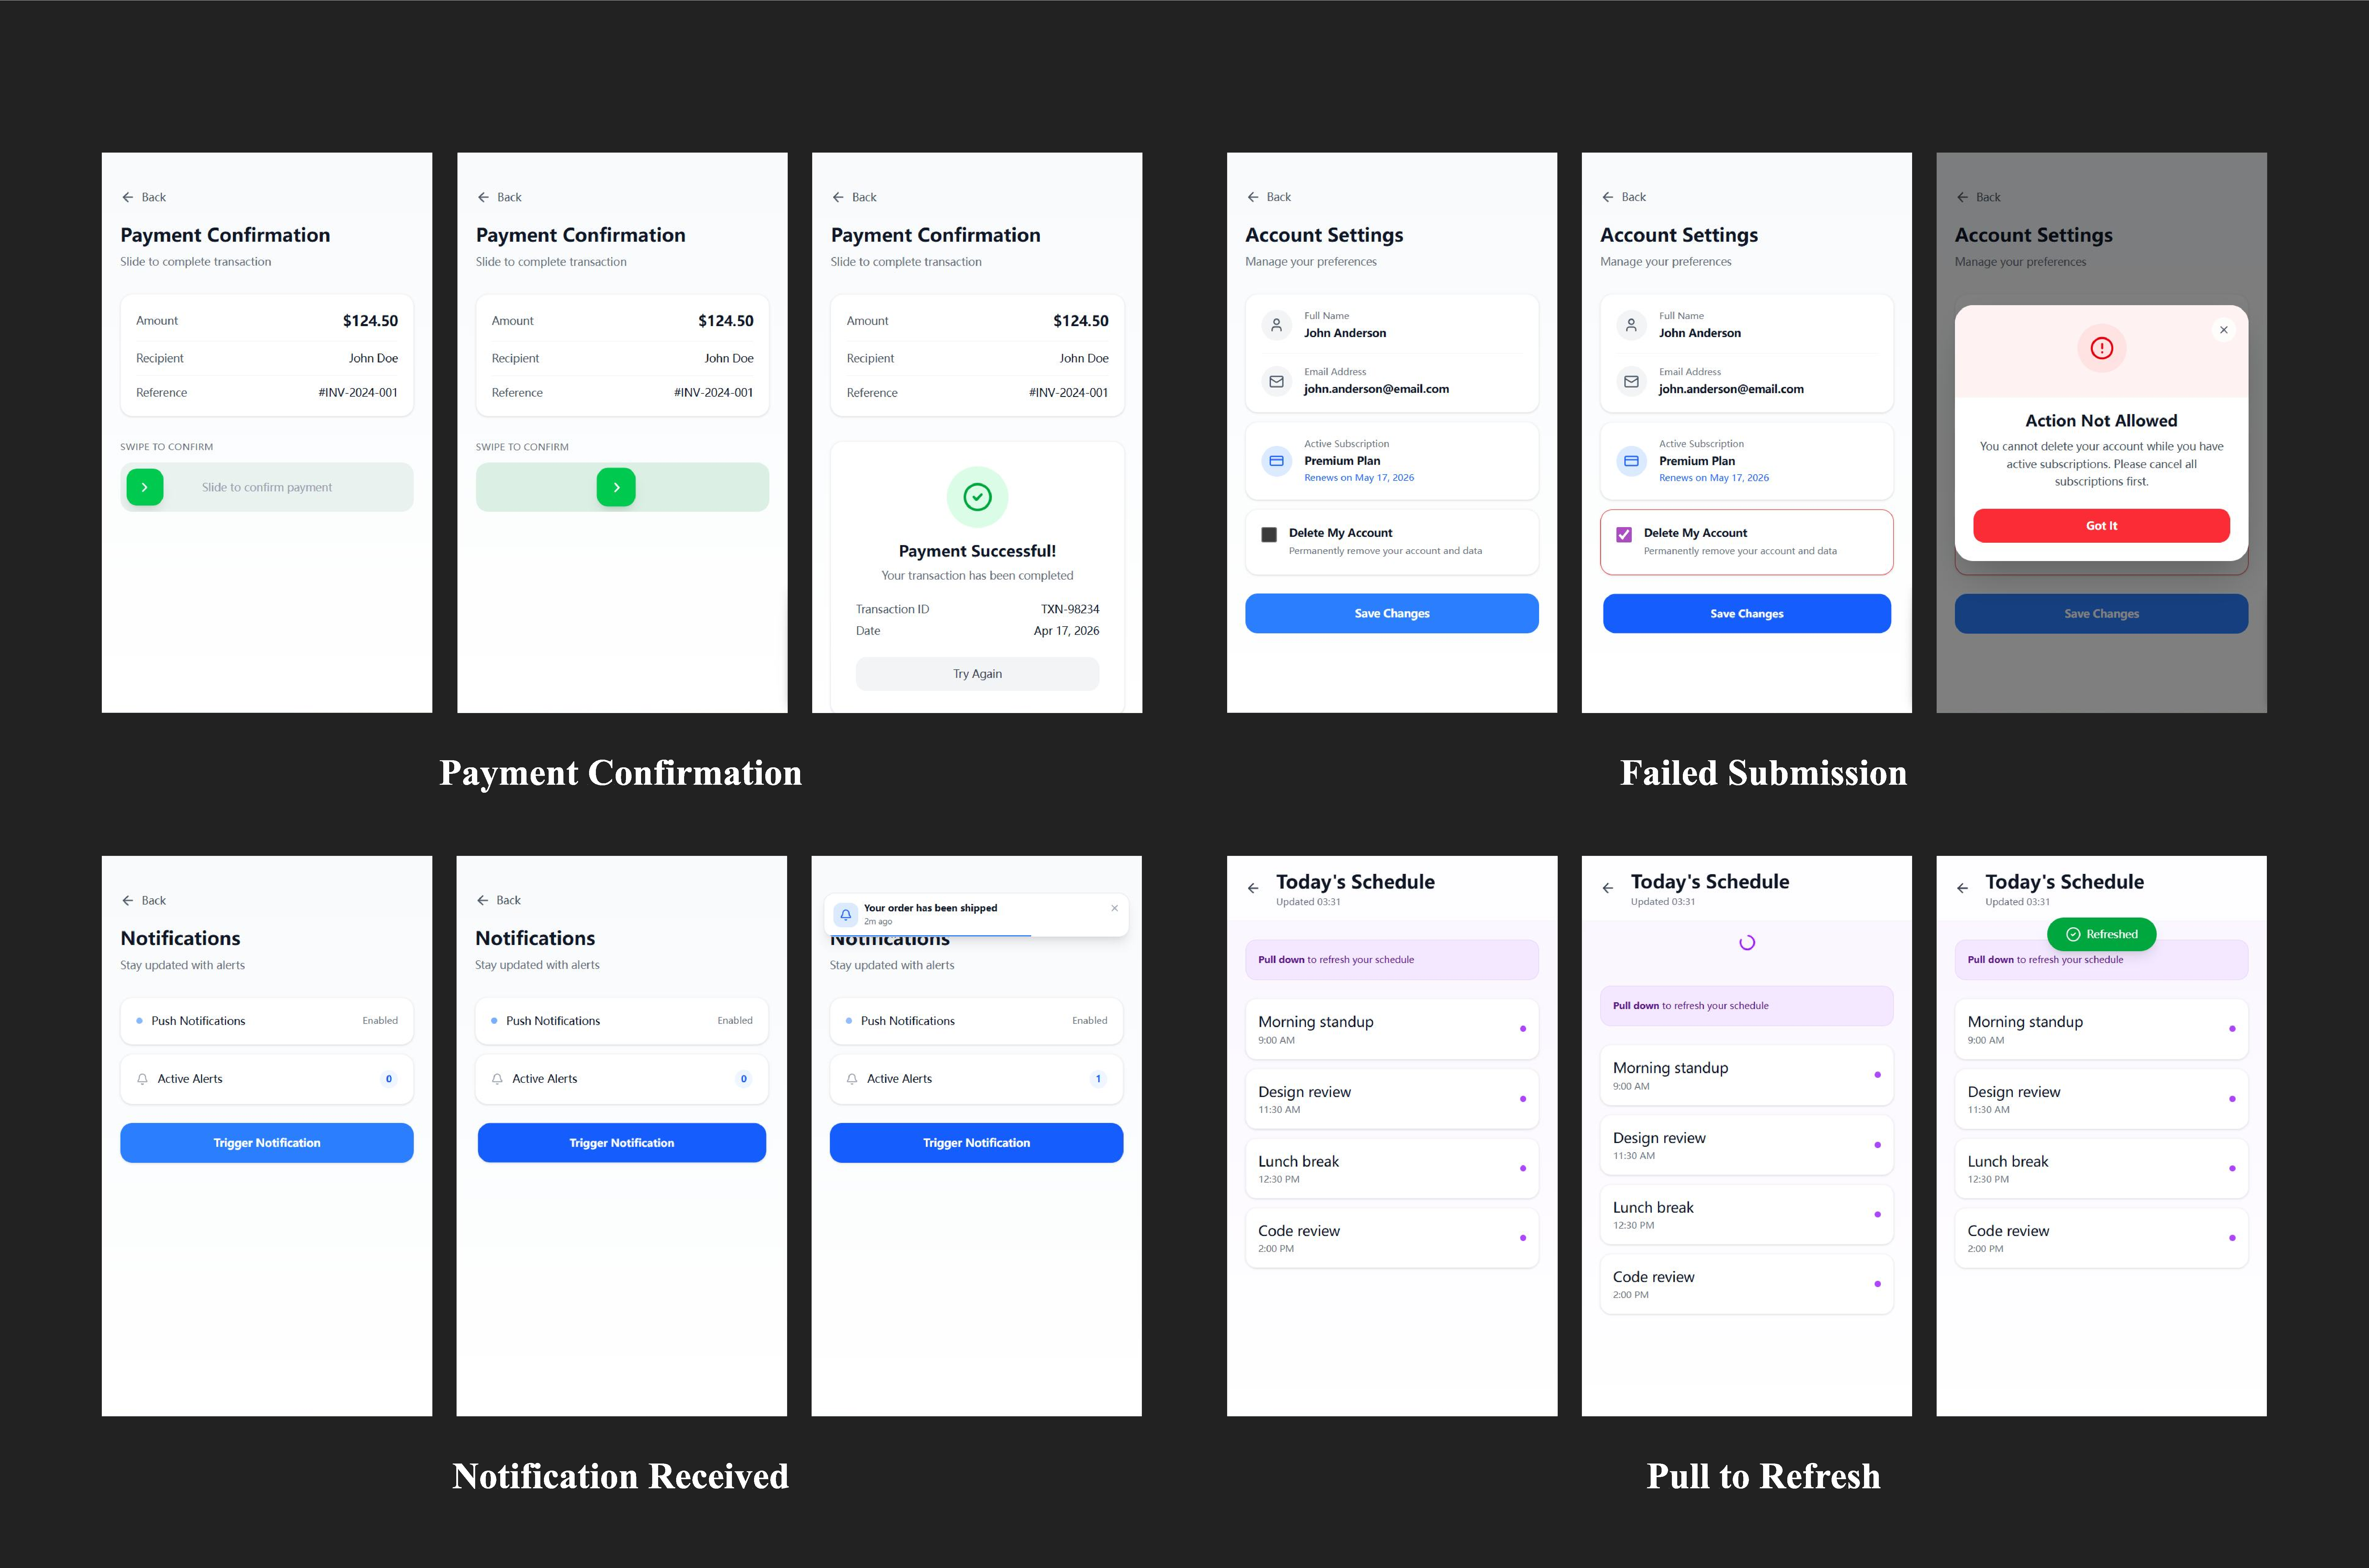
\includegraphics[width=\textwidth]{Figures/study_ui_flows.pdf}
\caption{Study UI flows.}
\label{fig:study-ui-flows}
\end{figure}

The Payment Confirmation flow shows a user sliding to confirm a payment, followed by a successful payment state. It represents a positive closure event in which haptic feedback should support a sense of completion, confidence, and confirmation. The Failed Submission flow shows a user clicking a control and receiving an error message. It represents a two-stage event in which an input action is followed by a later system refusal, making temporal separation and error salience important. The Notification Received flow shows a user pressing a trigger button and then receiving a message notification. It tests whether haptic feedback can indicate arrival or attention without feeling overly disruptive. The Pull to Refresh flow shows a downward pull gesture, a loading state, and a refreshed completion cue. It emphasizes process, motion, and completion across a longer temporal sequence.

Each flow was shown as an animated visual sequence. Within a flow block, the visual sequence was held constant while the haptic stimulus varied. This design allowed participants to compare how different vibrations fit the same temporal visual event. Each flow block contained 15 anonymous haptic stimuli, and the full study included 60 haptic stimuli across the four flows. The next section describes the generation methods represented within each set of 15 stimuli.

\section{Compared Generation Methods}

The study compared five haptic generation methods, summarized in Table~\ref{tab:generation-methods}. For each UI flow, each method contributed three variants, producing 15 anonymous stimuli per flow and 60 stimuli in total. All methods produced a two-second sequence at 10 ms intervals before being converted through the shared ERM preprocessing and playback pipeline described in Chapter 3. Except for Random Noise, the methods used the same OpenAI 4.1 model as the upstream language or vision-language component. This controlled the LLM component of the comparison while varying how its output was used for haptic generation.

\begin{table}[t]
\centering
\caption{Compared generation methods.}
\label{tab:generation-methods}
\small
\setlength{\tabcolsep}{3pt}
\renewcommand{\arraystretch}{1.15}
\begin{tabular}{@{}>{\raggedright\arraybackslash}p{1.05in}>{\raggedright\arraybackslash}p{1.6in}>{\centering\arraybackslash}p{0.6in}>{\centering\arraybackslash}p{0.9in}>{\raggedright\arraybackslash}p{1.3in}@{}}
\hline
\textbf{Method} & \textbf{Input / control signal} & \textbf{Uses VAE?} & \textbf{Uses visual event semantics?} & \textbf{Purpose in comparison} \\
\hline
Random Noise & Random 2 s sequence & $\times$ & $\times$ & Unstructured random baseline \\
Random-Plan VAE & OpenAI-generated random event plan & \checkmark & $\times$ & Structured but UI-agnostic VAE baseline \\
HapticGen & OpenAI-generated text prompt from UI images & $\times$ & \checkmark & Prompt-based generative haptic baseline \\
Direct LLM Pattern & OpenAI-authored 10 ms sequence from UI images & $\times$ & \checkmark & Direct actuator-sequence baseline \\
Semantic VAE & OpenAI-generated semantic event plan from UI images & \checkmark & \checkmark & Proposed UI-grounded semantic VAE method \\
\hline
\end{tabular}
\end{table}


Random Noise generated a fully random two-second vibration sequence. It provided the lowest-level baseline: a stimulus with no visual grounding, no semantic event structure, and no learned haptic waveform prior. This condition tested whether participants were responding to structured haptic design rather than arbitrary vibration energy.

Random-Plan VAE used the same downstream VAE generation pipeline as Semantic VAE, but its event plan was not grounded in the UI flow. The OpenAI 4.1 model was used to produce a random schema-valid haptic event plan, including behavior class, semantic role, style, strength, timing hint, duration hint, and prototype anchor. The plan was then passed through semantic target feature construction, atlas-guided latent search, VAE decoding, timeline mixing, and ERM export. This condition corresponds to the Random VAE condition in the study data, but it is more precisely described as a random-plan VAE baseline: it tests a structured but UI-agnostic version of the pipeline.

HapticGen served as a prompt-based generative haptic baseline. For each variant, the same UI flow images were first used to generate a text prompt through the OpenAI 4.1 model, and that prompt was then used as the input to HapticGen. The resulting waveform was converted to the same two-second sequence format and passed through the same ERM preprocessing pipeline as the other methods.

Direct LLM Pattern tested whether a language model could directly author a usable actuator-oriented sequence from the visual event. For each UI flow variant, the before, during, and after images were given to the OpenAI 4.1 model with instructions to output a two-second ERM-oriented sequence at 10 ms intervals. This method therefore used the visual event input but bypassed the VAE, behavior atlas, latent search, and timeline mixer.

Semantic VAE was the proposed method. It used the OpenAI 4.1 model to convert the UI flow images into a semantic haptic event plan and then generated the final stimulus through the behavior atlas, semantic-feature-guided latent search, VAE decoding, event timeline mixing, and shared ERM export. Compared with Random-Plan VAE, it tests the value of grounding the semantic event plan in the visual event. Compared with HapticGen and Direct LLM Pattern, it tests the value of separating visual-event interpretation from waveform generation through an explicit semantic intermediate representation and a learned haptic latent space.

\section{Study Procedure}

The user study used a within-subject design with 27 participants. Each participant experienced all four UI flow blocks and all five generation methods. This design allowed each participant to serve as their own comparison point across methods, reducing the effect of individual differences in haptic sensitivity and preference.

The study was organized into four flow blocks presented in a fixed order: Payment Confirmation, Failed Submission, Notification Received, and Pull to Refresh. Each block contained 15 anonymous haptic stimuli, corresponding to three variants from each of the five generation methods. Within a block, the visual flow was fixed and the anonymous card positions were randomized by a seed. Participants saw only anonymous IDs, so method labels were hidden throughout the study.

Participants completed each block at their own pace. They could click the anonymous haptic cards in any order, replay any stimulus as many times as they wanted, and revise their ratings before leaving the block. Triggering a card replayed the animated UI flow and the corresponding ERM vibration together. For each stimulus, participants gave two 7-point Likert ratings: whether the haptic clearly conveyed a meaningful response and whether it fit the visual event.

After rating the 15 stimuli in a block, participants completed a block-level comparison on the same page. They selected one to three haptics that were the best overall matches for the flow and one to three haptics that were the worst overall matches. Participants could replay stimuli while making these choices and could optionally provide text explanations for why the selected haptics were stronger or weaker fits.

Participants were allowed to pause or rest at any point. Most sessions were completed in approximately 30 minutes, while some sessions lasted up to about one hour depending on how often participants replayed stimuli and revised their responses. After completing the panel, participants filled out a follow-up survey. The survey did not collect demographic variables such as age or gender; instead, it asked about study-relevant background, including frequency of electronic-device use and how often participants notice haptic feedback in everyday devices.

\section{Measures and Analysis Plan}

The study produced three main forms of evidence: per-stimulus Likert ratings, within-flow best and worst selections, and open-text explanations. These measures were designed to capture both absolute judgments of individual stimuli and comparative preferences within the same visual event context.

For each stimulus, participants provided two 7-point Likert ratings. The first measured whether the haptic stimulus clearly conveyed a meaningful response, and the second measured whether the haptic stimulus fit the visual event. In the results analysis, ratings are summarized at the participant level for each method and flow by averaging across the three variants produced by the same method. This preserves the within-subject structure of the study and avoids treating multiple variants from the same participant and condition as independent observations. Chapter 5 reports descriptive statistics by method and flow and uses repeated-measures comparisons where appropriate, with non-parametric tests such as Friedman tests and corrected post-hoc comparisons used for method-level contrasts.

The best and worst selections provide a second measure of relative preference. Because participants selected one to three strongest and weakest matches within each flow, these responses reflect direct comparison among stimuli shown under the same visual event. Anonymous stimulus IDs are mapped back to generation methods using the stimulus key, and the analysis reports selection counts and proportions by method and flow. These counts complement the Likert ratings by showing which methods were repeatedly chosen as especially strong or especially weak matches.

Open-text explanations are analyzed using qualitative content analysis. Responses are coded with an explicit codebook covering themes such as semantic fit, timing and rhythm, intensity, smoothness, randomness, progress, comfort, and subtlety. A single response may receive multiple theme codes when it refers to more than one perceptual or semantic property. The qualitative analysis is used to interpret the rating and selection patterns rather than to replace them. The follow-up survey is used descriptively to contextualize participants' familiarity with electronic devices and everyday haptic feedback.

\chapter{Results}

[TODO: draft this chapter after confirming the statistical analysis plan for the four user study CSV files.]

\chapter{Discussion and Conclusion}

[TODO: draft this chapter after interpreting the final quantitative and qualitative findings.]


\appendix
\chapter{System Configuration Details}
\label{app:system-config}

\section{VAE Training Configuration}
\begin{table}[p]
\centering
\small
\caption{Full VAE training configuration.}
\label{tab:vae-full-config}
\renewcommand{\arraystretch}{1.05}
\begin{tabular}{@{}>{\raggedright\arraybackslash}p{1.25in}>{\raggedright\arraybackslash}p{1.65in}>{\raggedright\arraybackslash}p{2.35in}@{}}
\hline
\textbf{Category} & \textbf{Parameter} & \textbf{Value} \\
\hline
Dataset & Source & HapticGen WAV files \\
Dataset & Number of WAV files & 793 \\
Dataset & Train / validation split & 634 / 159 \\
Input representation & Chunk duration & 0.5 s \\
Input representation & Sampling rate & 8 kHz \\
Input representation & Samples per chunk & 4000 \\
Preprocessing & Segment selection & Energy-rich segment sampling \\
Preprocessing & Global RMS & 0.0487 \\
Preprocessing & Normalization & Global RMS normalization, scale 0.25 \\
Preprocessing & Clipping range & $[-5, 5]$ \\
Preprocessing & Min--max normalization & Disabled \\
Augmentation & Gain range & 0.8--1.2 \\
Augmentation & Temporal shift & Up to 64 samples \\
Augmentation & Noise / dropout & Disabled \\
Model & Architecture & Conv1D VAE \\
Model & Latent dimension & 12 \\
Model & Encoder channels & 64, 128, 256, 256 \\
Model & Activation / normalization & Leaky ReLU / group normalization \\
Training & Batch size & 16 \\
Training & Maximum epochs & 600 \\
Training & Early stopping patience & 60 \\
Training & Optimizer learning rate & 0.0003 \\
Loss & Time-domain reconstruction & MSE + 0.3 L1, weighted by 2.2 \\
Loss & Multi-scale STFT & Enabled at scales 32, 64, 128, 256 \\
Loss & STFT scale weights & 1.6, 1.3, 0.9, 0.5 \\
Loss & STFT linear / log weights & 0.06 / 0.03 \\
Loss & Amplitude weight & 0.25 \\
Loss & Temporal derivative weight & 0.15 \\
Loss & Event envelope weight & 0.4 \\
Loss & Event local RMS weight & 0.8 \\
Loss & Event onset weight & 0.2 \\
Loss & Event analysis windows & 16, 32, 64, 128, 256 \\
Loss & KL maximum beta & 0.0002 \\
Loss & Free bits & 0.03 \\
\hline
\end{tabular}
\end{table}


\section{Latent Search Configuration}
\begin{appendixtable}
\centering
\caption{Latent search stages.}
\label{tab:latent-search}
\begin{singlespace}
\renewcommand{\arraystretch}{1.1}
\begin{tabular}{@{}>{\raggedright\arraybackslash}p{1.65in}>{\raggedright\arraybackslash}p{4.15in}@{}}
\hline
\textbf{Stage} & \textbf{Operation} \\
\hline
Target construction & Convert semantic event fields into target waveform features. \\
Anchor selection & Select four nearest curated atlas prototypes within the requested behavior class. \\
Anchor weighting & Weight anchors by inverse feature distance. \\
Initial latent estimate & Compute a weighted average of anchor latent vectors. \\
Candidate sampling & Sample 32 latent candidates near the initial estimate using strength-scaled noise. \\
Candidate decoding & Decode each candidate with the VAE decoder. \\
Feature scoring & Compare decoded waveform features with the semantic target features. \\
Latent selection & Select the best-scoring candidate as \texttt{generated\_raw\_z}. \\
\hline
\end{tabular}
\end{singlespace}
\end{appendixtable}


\section{Timeline Mixer Configuration}
\begin{table}[t]
\centering
\caption{Timeline mixer parameters.}
\label{tab:timeline-mixer}
\renewcommand{\arraystretch}{1.1}
\begin{tabular}{@{}>{\raggedright\arraybackslash}p{1.9in}>{\raggedright\arraybackslash}p{3.9in}@{}}
\hline
\textbf{Parameter} & \textbf{Value or role} \\
\hline
Final duration & 2.0 s \\
Sample rate & 8 kHz \\
Final waveform length & 16000 samples \\
Default event gap & 0.08 s \\
Minimum event gap & 0.02 s \\
Minimum event duration & 0.35 s \\
End alignment point & 1.9 s \\
Duration mode & Hold-stretch \\
Mixer mode & Additive \\
Fade & 10 ms at event boundaries \\
Final clip range & $\pm 3.0$ in the final stimulus run \\
Strength gain & $g = 0.5 + 0.8s$ \\
Sequence export & 10 ms interval; 200 values over 2.0 s \\
\hline
\end{tabular}
\end{table}


\section{ERM Preprocessing Configuration}
\begin{appendixtable}
\centering
\caption{ERM preprocessing parameters.}
\label{tab:erm-preprocessing}
\begin{singlespace}
\renewcommand{\arraystretch}{1.1}
\begin{tabular}{@{}>{\raggedright\arraybackslash}p{1.9in}>{\raggedright\arraybackslash}p{3.9in}@{}}
\hline
\textbf{Parameter} & \textbf{Value or role} \\
\hline
Input duration & 2.0 s \\
Input interval & 10 ms \\
Input length & 200 values \\
Output interval & 20 ms \\
Output length & 100 values \\
Resampling & Peak-hold max pooling \\
Threshold & 20 \\
Gamma & 0.65 \\
Minimum nonzero drive & 35 \\
Maximum drive & 220 \\
Minimum pulse length & 3 output frames \\
Attack smoothing & 1 output frame \\
Release smoothing & 2 output frames \\
Shared preprocessing & Applied to all five user-study methods \\
\hline
\end{tabular}
\end{singlespace}
\end{appendixtable}



%%%%%%%%%%%%%%%%%%%%%%%%%%%%%%%%%%%%%%%%%%%%%%%%%%
% Back Matter
%%%%%%%%%%%%%%%%%%%%%%%%%%%%%%%%%%%%%%%%%%%%%%%%%%
\backmatter

\bibliographystyle{amsplain}
\addcontentsline{toc}{chapter}{References}
\bibliography{Bibliography/references}
\markboth{{\rmfamily\scshape Bibliography}}{}

\end{document}
